%%
%% This is file `sample-acmsmall.tex',
%% generated with the docstrip utility.
%%
%% The original source files were:
%%
%% samples.dtx  (with options: `acmsmall')
%% 
%% IMPORTANT NOTICE:
%% 
%% For the copyright see the source file.
%% 
%% Any modified versions of this file must be renamed
%% with new filenames distinct from sample-acmsmall.tex.
%% 
%% For distribution of the original source see the terms
%% for copying and modification in the file samples.dtx.
%% 
%% This generated file may be distributed as long as the
%% original source files, as listed above, are part of the
%% same distribution. (The sources need not necessarily be
%% in the same archive or directory.)
%%
%% The first command in your LaTeX source must be the \documentclass command.
\documentclass[acmsmall]{acmart}
%% NOTE that a single column version is required for 
%% submission and peer review. This can be done by changing
%% the \doucmentclass[...]{acmart} in this template to 
%% \documentclass[manuscript,screen]{acmart}
%% 
%% To ensure 100% compatibility, please check the white list of
%% approved LaTeX packages to be used with the Master Article Template at
%% https://www.acm.org/publications/taps/whitelist-of-latex-packages 
%% before creating your document. The white list page provides 
%% information on how to submit additional LaTeX packages for 
%% review and adoption.
%% Fonts used in the template cannot be substituted; margin 
%% adjustments are not allowed.
%%
%% \BibTeX command to typeset BibTeX logo in the docs
\AtBeginDocument{%
  \providecommand\BibTeX{{%
    \normalfont B\kern-0.5em{\scshape i\kern-0.25em b}\kern-0.8em\TeX}}}

%% Rights management information.  This information is sent to you
%% when you complete the rights form.  These commands have SAMPLE
%% values in them; it is your responsibility as an author to replace
%% the commands and values with those provided to you when you
%% complete the rights form.
\setcopyright{acmcopyright}
\copyrightyear{2021}
\acmYear{2021}
\acmDOI{10.1145/1122445.1122456}


%%
%% These commands are for a JOURNAL article.
%% ICTD commenting these
%%\acmJournal{JACM}
%%\acmVolume{37}
%%\acmNumber{4}
%%\acmArticle{111}
%%\acmMonth{8}

%%
%% Submission ID.
%% Use this when submitting an article to a sponsored event. You'll
%% receive a unique submission ID from the organizers
%% of the event, and this ID should be used as the parameter to this command.
%%\acmSubmissionID{123-A56-BU3}

%%
%% The majority of ACM publications use numbered citations and
%% references.  The command \citestyle{authoryear} switches to the
%% "author year" style.
%%
%% If you are preparing content for an event
%% sponsored by ACM SIGGRAPH, you must use the "author year" style of
%% citations and references.
%% Uncommenting
%% the next command will enable that style.
%%\citestyle{acmauthoryear}

\usepackage{listings}
\lstset{basicstyle=\tiny}

%%
%% end of the preamble, start of the body of the document source.
\begin{document}

%%
%% The "title" command has an optional parameter,
%% allowing the author to define a "short title" to be used in page headers.
\title{Scheduling Musical Events in Max/MSP with Scheme For Max}

%%
%% The "author" command and its associated commands are used to define
%% the authors and their affiliations.
%% Of note is the shared affiliation of the first two authors, and the
%% "authornote" and "authornotemark" commands
%% used to denote shared contribution to the research.
\author{Iain C.T. Duncan}
%%\authornote{Both authors contributed equally to this research.}
\email{iduncan@uvic.ca}
\affiliation{
  \institution{University of Victoria}
  %%\streetaddress{}
  \city{Victoria}
  \state{BC}
  \country{Canada}
  %%\postcode{V8P 5C2}
}


%%
%% By default, the full list of authors will be used in the page
%% headers. Often, this list is too long, and will overlap
%% other information printed in the page headers. This command allows
%% the author to define a more concise list
%% of authors' names for this purpose.
\renewcommand{\shortauthors}{Duncan}

%%
%% The abstract is a short summary of the work to be presented in the
%% article.
\begin{abstract}
Scheme For Max (S4M) is an open source project that enables embedding 
s7 Scheme interpreters in the Max/MSP visual programming environment,
the most widely adopted programming platform for computer music.
Of particular note is its appropriateness for flexibly
and accurately scheduling future musical events, a capability not
adequately supported thus far in Max. This is accomplished by scheduling
Scheme procedures integrated with the Max scheduler, and the 
implementation of this facility is discussed.
In addition to scheduling, S4M enables users of Max to script Max 
generally in Scheme and provides facilities for 
real-time dynamic code evaluation (a.k.a. ``live-coding") within the
Max environment. 

\end{abstract}

%%
%% The code below is generated by the tool at http://dl.acm.org/ccs.cfm.
%% Please copy and paste the code instead of the example below.
%%

\begin{CCSXML}
<ccs2012>
<concept>
<concept_id>10010405.10010469.10010475</concept_id>
<concept_desc>Applied computing~Sound and music computing</concept_desc>
<concept_significance>500</concept_significance>
</concept>
<concept>
<concept_id>10010405.10010469.10010474</concept_id>
<concept_desc>Applied computing~Media arts</concept_desc>
<concept_significance>500</concept_significance>
</concept>
</ccs2012>
\end{CCSXML}

\ccsdesc[500]{Applied computing~Sound and music computing}
\ccsdesc[500]{Applied computing~Media arts}
%%
%% Keywords. The author(s) should pick words that accurately describe
%% the work being presented. Separate the keywords with commas.
\keywords{music computing, event scheduling, live-coding}

%%
%% This command processes the author and affiliation and title
%% information and builds the first part of the formatted document.
\maketitle

\section{Introduction}

Max (also known as Max/MSP) is a programming environment for creating interactive 
music and multi-media programs through a visual programming language accessible 
to non-programmers. Max was created to make it possible for users
to go beyond the limits of commercial music sequencing tools, creating
interactive environments of arbitrary complexity and sophistication
\cite{Zicarelli2002}.
Programs, or ``patches" in the Max nomenclature, are created by placing
visual boxes representing Max objects on a canvas and connecting them visually with
``patch cords", a paradigm similar to that of modular synthesizers and familiar to many musicians.
First created in the mid 1980's by Miller Puckette while at IRCAM 
(Institut de recherche et coordination acoustique/musique), 
Max is now developed and sold by the San Francisco software company Cycling '74,
and is widely used in both academic and commercial music contexts as well
as in multi-media installations. A rich library of Max objects exists, 
both provided with Max and available as open-source 
extensions, enabling users to rapidly create interactive systems with gestural 
input from physical sources such as on screen widgets, physical electronic instruments,
and custom hardware communicating over serial networks.

\begin{figure}[h]
  \centering
  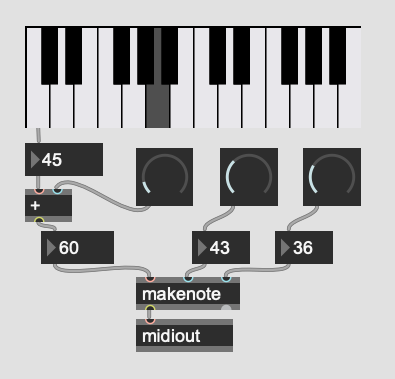
\includegraphics[width=.5\linewidth]{fig-1}
  \caption{A Max patch with a keyboard value transposed by a dial and sent to MIDI output.}
  \Description{}
\end{figure}


One powerful feature of Max is its ability to be programmed
while the engine is playing music. Patches can be altered 
without necessarily interrupting patch activity (depending on the design
of the program), and this can
even be performed live, an activity known as ``live-coding", which has
emerged since the early 2000's as its own musical sub-culture of 
live programming performances
with tools such as Max, SuperCollider, Csound, and others \cite{Roberts18}.
This approach to music making overlaps with the related discipline of 
algorithmic music, in which programmatic algorithms are used
not just for affecting musical parameters such as volume, pitch, and timbre, 
but also for the generation of musical content such as melodies
and rhythms.

In both the fields of live-coding and algorithmic music, the ability for
the performer and composer to schedule events in the future with high temporal
accuracy is of major benefit. A common scenario is that a solo performer or duo
is composing electronic music on the fly for a large number of voices --- more than
the performers have hands. Thus they create abstractions of musical content,
and request from the system that potentially many of these will begin together
at some point in the future. For example, a performer may program a drum
groove that has a large number of interacting lines, but wish the groove
to only begin playing, and thus be audible, at the beginning of the next 16-bar 
musical boundary. While this is possible in the Max visual
patching language, it is cumbersome and thus the implementation is not
optimal for live-coding or algorithmic music where the speed with which
the user can accomplish this is an important consideration. In a live
electronic music context, one of the primary challenges for the perfomers
is the design of a working system that enables them to create new material on
stage (making the performances engaging and improvisatory), 
but in a way that enables them to work fast enough not to bore an audience!

In addition to the Max visual patching language, Max can be programmed
by creating new Max objects (``externals" in the Max nomenclature) in C or C++ 
using the Max SDK and API, and can also be programmed in text-based 
languages through regular Max objects that themselves provide embedded language
interpreters. Max provides one such interpreter in the \textbf{js} object, 
which embeds a JavaScript interpreter, and others contributed by third parties
exist for languages such as for Lua, Python, and Ruby. 

Scheme For Max (a.k.a. S4M) is an open-source external developed by the 
author that embeds the s7 Scheme interpreter, a Scheme dialect created by
Bill Schottstaedt at the  Center for Computer Research in Music and Acoustics
(CCRMA) at Stanford University. Originally developed
from TinyScheme, s7 is a Scheme dialect designed for use in computer music
platforms and is used in various music programs such as the Snd editor and the
Common Music algorithmic composition platform \cite{Schottstaedt2021}.
Similar in functionality to the built-in \textbf{js} object, 
the \textbf{s4m} object enables the user to program Max in s7 Scheme,
and provides Scheme functions to interact with the Max engine and environment through
a foreign function interface implemented in C using the Max C SDK and API.

The author believes that S4M extends Max in a way that is of significant value to 
the algorithmic musician and live-coding performer, as well as more generally 
to the broader Max community. The ability to update
a running Scheme program during playback is a major benefit
and is a capability that has been, while technically possible, impractical
with existing solutions such as JavaScript. Additionally, the syntax
of Scheme bears a convenient similarity to Max message syntax, and thus 
one can easily use Max visual widgets and messages to generate small Scheme programs in the
patcher. Potentially the most interesting benefit is the ease with which the user 
can create and schedule functions for evaluation in the future, with 
input into these functions coming from Max patching widgets, and flexible control
over the current and future evaluation context of the functions and variables used.

\begin{figure}[H]
  \centering
  \includegraphics[width=\linewidth]{fig-youtube.png}
  \caption{Demonstration of real-time algorithmic music by the author, in which S4M is used
  to control a Eurorack modular synthesizer. https://youtu.be/pg7B8h4yHkU \& https://youtu.be/rcLWTjN4qBI  }
  \Description{.}
\end{figure}


This paper provides an overview of the Max platform and the problem of musical scheduling
in computer music, as well as the existing Max solutions to this problem, 
and a discussion of the limitations of these solutions.
It then introduces Scheme For Max and examines how the use of Scheme
overcomes these limitations, and provides details of
the implementation of scheduling in S4M, both at the Scheme and
C programming levels. Finally, it concludes with discussion of 
the current limitations of, and future possibilities for, Scheme For Max. 

\section{Background - Programming Music in Max/MSP}

\subsection{The Max Environment}

Max is a visual programming environment for interactive multi-media, 
used widely in music academia as well as in commercial music circles through Max for Live, 
a version of Max embedded in the Ableton Live digital audio workstation. 
Max patches are created by placing visual boxes on a canvas 
and connecting them graphically with ``patch cords", where a box may be
any of the Max object types installed on the user's system. A box placed on the patcher
results in the instantiation of an object in memory from a prototypical class for the object, with
text fields typed in the visual patching box used as constructor arguments. 
Thus a Max patch consists of a collection of instantiated objects that send messages to each other
in a directed graph, producing a data-flow execution model whereby a message from a source 
object triggers execution in one or more 
receiving objects, who may in turn send on messages to other similarly connected objects. 

Patch activity, in the form of messages moving through the graph, can be initiated by 
various forms of real-time input, such as keyboard and mouse events, connected electronic instruments, and networking 
events, as well as by scheduled events through Max objects such as the \textbf{metronome}, which sends
out messages at regular time intervals. Messages are 
stored internally as lists of Max ``atoms", which may be symbols, integers, or floating point numbers 
\cite{Puckette2002}.
There also exists a Max object for visually displaying and altering messages called the \textbf{message-box},
which allows messages to be typed directly in the object in the visual patcher, and then sent by clicking the box.  
Execution follows a depth-first and right-to-left order, enabling the programmer to deterministically 
control the execution flow with the visual layout of the patch cords. (i.e., A source object sending 
messages out to multiple receiving sub-graphs results in the right-hand message path completing 
execution to the bottom before moving left, rather than spawning two concurrent threads of execution.) When 
patching, messages can be inspected by sending them to a \textbf{print} object (which prints to the Max console),
to a \textbf{message-box} object (which will update its visual display of the message) 
or through a built-in visual debugger using a feature Max calls ``probing”.

In addition to this event-based message execution model, also called ``control messages", Max 
supports a stream-based digital 
audio execution model, originally provided separately as a product called ``MSP", but now included 
as part of the single Max product.
MSP activity normally runs in a separate thread from the event/message Max operations, and uses 
a separate class of objects that pass constant streams of digital audio to each other through differently 
colored patch cords (though MSP objects may additionally receive control messages for controlling parameters). As  
S4M executes only at the event/message level and does not implement DSP operations, MSP is not 
discussed further here. 


\subsection{Max Message and Object Implementation} 

Internally, Max messages are data entities consisting of a symbol that acts
as a Smalltalk-style message selector and an optional array of Max atoms. 
Each atom entity contains a member for the atom type and another for its value, 
where the type may be any of \textbf{int,} \textbf{float,} or \textbf{symbol}. 
Note that while the message selector symbol is always present at the C level,
in the visual patcher the selector may be implicit and hidden from the user. 
(i.e., the message originating from a message box that appears to contain only an integer
will actually consist of the selector ``int" followed by an atom storing the numerical value.)
The symbol ``bang" is a special symbol that can be used for a one-element message 
that essentially means ``run", and the act of triggering execution by sending a bang
message from the \textbf{bang} object is called ``banging" in the nomenclature.
(Note that there are both messages and objects called ``bang"; the \textbf{bang} 
object is an object that sends a bang message on receipt of any message.)
Taken together, this means that in Max there are five kinds of messages: 
\textbf{bang}, \textbf{symbol}, \textbf{int}, \textbf{float}, and \textbf{list}. 
\cite{Puckette2002}
(The bang message is technically a symbol message
of ``bang", but this is essentially treated as a type of its own in the nomenclature.) 

Activity in an object (represented visually by a single visual box in the patch) is triggered
by sending the object a Max message, most commonly from an object connected to it
through a patch cord running to an ``inlet" of the object. 
In order for the receiving object to do anything, it must 
be sent a message with a message selector for which it has a bound method,
a situation referred to in the nomenclature as ``responding to the message". Most objects
have a principal activity that typically ends with outputting the result of their calculation, and this is
often triggered by sending the object a single \textbf{bang} message or by sending a value to 
their first, or ``hot", inlet. In addition, they may respond to other messages to change internal state
data or configuration --- for example the ``set" message is commonly implemented to update internal
state without outputting any result. The end result of object methods run on receipt of a message falls broadly
into three (non-exclusive) categories: the object may update some internal state, it may send a
message or messages out of its outlets, and it may cause a side effect in the broader
Max environment, such as printing to the console or updating a global data element such as
an audio buffer.

As an example, in the patcher screenshot in figure 3 we see a \textbf{message-box} object that will update
its state (and visual display) with the symbols ``hello" and ``world" when sent the message 
\textbf{set hello world}. Near it is a circular \textbf{bang} object, which when clicked will send the
\textbf{message-box} the \textbf{bang} message, causing it to output the message \textbf{list hello world}.
This message will be received by the \textbf{zl.len} object, which counts the number of elements 
in any lists it receives, immediately outputting the count. The three columns in the screen-shot
show the patch as it is prior to any clicks, as it is after clicking \textbf{message-box} 1,
and as it is after clicking both \textbf{message-box} 1 and the \textbf{bang}.

\begin{figure}[H]
  \centering
  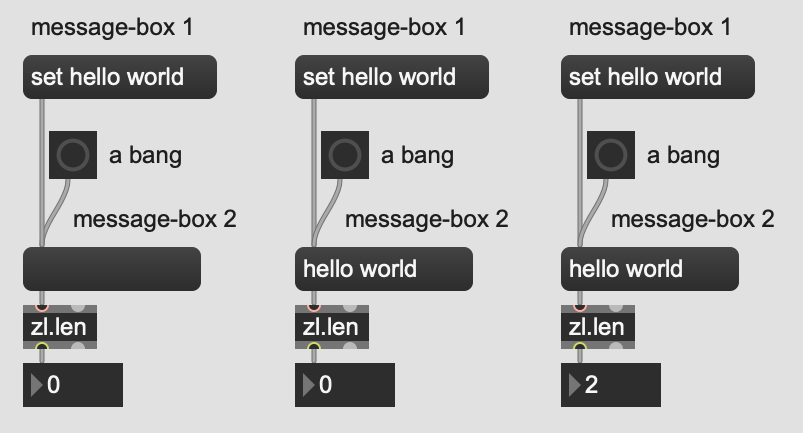
\includegraphics[width=.5\linewidth]{fig-2-message-flow}
  \caption{Message flow at three stages}
  \Description{.}
\end{figure}

Objects are not limited to interacting with other objects through messages passing into inlets and out of 
outlets. A C API exists that enables objects to query and control various engine components (e.g., 
the transport mechanism), and it is also possible for objects to send messages to other objects 
directly or through the scheduler queues, without the sending and receiving objects 
necessarily being connected visually in the patcher. Fundamentally however, the same mechanism
is used --- when an object calls a method on another object at the C level, this is still done
by creating a data structure of a message selector and optional atom arguments, 
and then sending this to the receiving object through a generic message sending function.

As each visual box in a patcher has state that is retained between messages, we can see that when
programming the visual patcher (a.k.a. ``patching"), we are in effect programming with
object instantiations rather than classes. In fact, in the Max engine, the act of creating
a new visual-box and placing it on the patcher canvas does indeed instantiate an object, creating
a fresh copy of the prototype's data structure and adding it to a graph of other objects.
This is in contrast to computer music languages such as Csound, where the user programs instruments 
with functions and the engine creates an instantiated data structure on each note-event sent to 
the instrument from a score --- in effect the instruments act as object builders and note-events 
become objects that exist for the duration of the note played \cite{Lazzarini2013}.

\subsection{Max Externals}

While Max is a commercial, closed-source product, it includes a software development kit for 
extending Max by writing a Max “external”. An external is a compiled plug-in that defines the  
prototype (data structure and methods) used to create new objects in the patcher.  
Externals are developed in C or C++ in an object-oriented manner, the C API using data 
structures and pointers to simulate class-based programming with dynamic binding,
and the more recent C++ API using C++ classes \cite{Zicarelli2002}.
A typical external will implement a class that provides some object state for instantiated
objects along with constructor and destructor functions, and  
methods for sending and receiving Max messages through the object’s inlets and outlets.
Methods are bound dynamically to the object prototypes.
The SDK and API also provide a rich body of functions for interacting with the overall Max
environment, thus these methods may also trigger side-effects through these facilities.

As externals are compiled plug-ins, they do not need to be distributed as source-code, and
are most typically made available as binaries for Windows and macOS. Extending Max through externals has 
been possible since very early versions of Max in the late 1980's,
thus thousands of 3rd party externals 
now exist \cite{MaxObjects2021}, both open and closed source, of which Scheme For Max is one.


\subsection{Lisp in Computer Music}

Scheme For Max is far from the first Lisp-based computer music tool, or even
the first real-time music tool in Lisp. There is a rich history of Lisp in music, 
including (but not limited to) Common Lisp Music, created by Bill Schottstaedt in the late 1980's
\cite{Wang17}, Heinrich Taube's Common Music from 1991 \cite{Taube91},
Roger Dannenberg's Nyquist from 1997 \cite{Dannenberg97},
and Andrew Sorensen's Impromptu from 2005 (later rewritten as Extempore) \cite{Sorensen2010}. 
Nor is Scheme For Max unique in providing a Lisp-family
extension facility to a larger music platform --- the author unknowingly
programmed in Lisp in the early 1990's while using the Cakewalk sequencer,
which came with an embedded Lisp interpreter in the form of the 
Cakewalk Application Language! There also exist Lisp-family client interfaces
to the open-source SuperCollider music platform, including Overtone (Clojure),
rsc3 (r6rs Scheme), and cl-collider (Common Lisp).

However, Scheme For Max is unique in bringing a fully-fledged Scheme interpreter
to the Max environment as a first-class Max object, implemented and running
identically to any built-in object. This is significant in that Max
is arguably the most widely used truly programmable
music platform, and certainly the most widely deployed through its use in 
the very successful Ableton Live digital audio workstation, as Max For Live.

In contrast with S4M, systems such as Common Lisp Music, Common Music, Nyquist, and Extempore
all run as stand-alone applications, with events originating from them either
rendered as audio internally or destined for other systems for rendering to audio. 
While these systems are, like Max, also capable
of receiving gestural input, they must, in essence, ``be their own boss" --- they provide
their own scheduler and timing clocks and act as the principal engine from which temporal
events originate. If they are to be used alongside another temporal engine, the two
must be synchronized and events sent back and forth over network connections of some kind.

There have also been previous Max externals created to allow one to use Lisp in Max in various ways.
Brad Garton authored MaxLispJ, an external that provides a Common Lisp interpreter 
(Armed Bear Common Lisp) embedded through the Java runtime that can be used within Max 
via the \textbf{mxj} object \cite{Garton2011}.
MOZ'Lib, by Julien Vincenot, takes another approach, in which the Max external
acts as a proxy to an externally running Steel Bank Common Lisp process,
a similar approach to that used by Cycling '74 for their \textbf{Node for Max} object (for Node.JS/ECMA6), 
thus enabling the outside process to execute long-running work without blocking Max \cite{Vincenot2017}.

In contrast to these, S4M embeds a light-weight Scheme interpreter directly in a Max
C external with no intermediate or external runtime necessary. This is made possible by the suitability
of Scheme for the creation of small, portable, and self-contained interpreters.
The s7 interpreter is implemented entirely in ANSI C, is statically linked during compilation of S4M, 
and operates entirely in whatever thread it is run in by the C host.
This means multiple instantiations of the interpreter are possible, and
each \textbf{s4m} object has direct C-level access to the Max C API 
through foreign function interface calls, with the results of said calls being exactly 
the same as if the functions were called in C, save execution time. 
The ramification of this is that S4M is unique among Max Lisp projects in being
able to operate within the native Max scheduling system, enabling highly accurate
timing and retaining deterministic control flow within a patcher. (i.e., There
is no hidden networking layer with communication to an outside process, which 
makes operations fundamentally asynchronous even if this is hidden from the user visually,
as is the case with Node for Max and MOZ'Lib.)
This provides the user with opportunities to use Scheme for tasks beyond
what is possible with previous options. 

For example, we are in effect 
able to say ``at a certain time, read some shared state and update an 
internal engine parameter accordingly". In the example below, a Scheme function
is scheduled that will, in 4 bars time, read a rehearsal mark from the table \textbf{mark-table},
advancing the global transport to that position. As the table
is a shared data object, other Max objects (or patchers) could write to this
rehearsal mark table without awareness of S4M. (Note: this is a safe operation
from Scheme code as table access is done through thread-safe Max SDK functions 
that handle synchronization and locking for us.)

\begin{figure}[H]
  \centering
  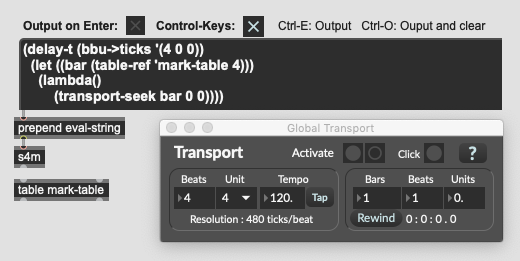
\includegraphics[width=.75\linewidth]{fig-3-transport}
  \caption{S4M patch that moves the transport in 4 bars time to a mark read from a table}
  \Description{.}
\end{figure}


\section{rationale for the choice of s7 scheme}

The design of the Max external system means that, technically, any interpreter
that can be embedded in a C host could be used. The author evaluated several during
the initial prototyping stages of development, including ECL (Embeddable Common Lisp),
Gambit, Chicken, Racket, Guile, and s7. The choice to use s7 was based on several 
factors, including the ease of embedding, its license, and its use in other computer music tools (and
thus its design suitability for computer music).

The s7 interpreter is implemented in a single C file (with header file), 
and is statically linked with the C code of the \textbf{s4m} object. Embedding is
as simple as linking to the s7 library and including a single file. In this 
regard (ease of embedding), it is similar to Guile, and in fact, is linguistically similar to Guile 1.8.
However, while Guile is licensed with the (somewhat reciprocal) LGPL license, s7 is liberally licensed 
under the BSD license. As the creation and sale of commercially externals is part of the Max 
milieu, the author felt this was more likely to result in uptake within the Max community.

Racket, Chicken, and Gambit were also potential contenders. In all three cases, the
complexity of embedding was significantly higher, and in at least one case (Chicken),
thread-safety for multiple interpreters in the same Max patch appeared problematic.
In addition, documented examples of common embedding use cases were less available
than with s7.

Finally, s7 was created for computer music, and as a result is used in other computer music
environments, such as Common Music. As a result, there is a rich body of code, especially
from Common Music, that can be used or studied by users. There is also a small, but active, 
online community of music programmers using s7, communicating through the CM-dist mailing
list hosted at the Stanford computer music center, CCRMA. The author of s7, Bill
Schottstaedt, has been working with Lisp and music since the 1980's, and has been an 
enthusiastic supporter of the project, providing invaluable suggestions and 
technical assistance.   


\section{implementation of the Scheme For Max external}

This section provides a high-level overview of the implementation of the \textbf{s4m} 
object provided by the Scheme For Max external.

The s7 foreign function interface enables one to define new Scheme functions in C 
for calling into C from Scheme, and to call any Scheme code from C. 
The interpreter is instantiated
in the \textbf{s4m} object's constructor (\textbf{s4m\_new} as per the Max naming conventions), and
a reference to it is stored in the \textbf{s4m} object's data structure.
Additionally, during initialization the external creates a Scheme-side variable 
that holds a pointer to the instantiated \textbf{s4m} object itself. Thus
both C functions that are called from Scheme and C functions called in response to Max
messages have access to both the \textbf{s4m} Max object and its associated s7 interpreter.
There is always one and only one s7 interpreter per \textbf{s4m} object instance, and
as s7 is thread safe, many \textbf{s4m} objects can be created in a Max patch, including
in both the low and high priority threads. (Max runs both a high-priority ``scheduler" 
thread and a low-priority ``UI" thread for event/message flow. Each \textbf{s4m} object 
runs in only one of these, chosen via an optional constructor argument, and incoming messages
from the opposite thread are deferred or promoted accordingly.)

Scheme-to-C calls are accomplished by defining a C function, and binding
it to a Scheme function name in the initialization routine. 
The function must take as arguments a pointer to the s7 interpreter instance and an \textbf{s7\_pointer}
that is a reference to a Scheme list of the arguments used in the Scheme call.
In the body of the function, C functions from the s7 API are used to get 
individual arguments from this list, the work is done for the function 
(which may include additional calls back into Scheme or Max API calls),
and finally, an \textbf{s7\_pointer} is returned, which becomes the return value of the 
function in Scheme.

C-to-Scheme calls are handled similarly: the C function (normally a method
of the \textbf{s4m} object that runs in response to a Max message) uses the
\textbf{s4m} object's reference to its s7 interpreter and the s7 API to build
Scheme argument lists and call into Scheme, getting back an \textbf{s7\_pointer} that
is then converted to one or more Max atoms. In both cases, helper
functions that convert Max atoms to s7 objects and vice versa are used, 
implemented as \textbf{max\_atom\_to\_s7\_obj} and \textbf{s7\_obj\_to\_max\_atom}
respectfully. The code example below shows sample functions for both directions.

\begin{lstlisting}[language=C]

// a C function that is called from Scheme as (post . args)
// it logs to the Max console through the Max API "post" function
static s7_pointer s7_post(s7_scheme *s7, s7_pointer args) {
    // all s7 functions have this form, args is a list, s7_car(args) is the first arg, etc 
    char *msg = s7_string( s7_car(args) );
    post("s4m: %s", msg);
    return s7_nil(s7);
}

// a C function that is called from Max (by a clock) and calls into Scheme
void s4m_clock_callback(void *arg){
    // use the clock info structure to get the delayed function handle
    t_s4m_clock_callback *ccb = (t_s4m_clock_callback *) arg;
    t_s4m *x = &(ccb->obj);
    t_symbol handle = *ccb->handle; 
    
    // create an argument list for calling into Scheme
    // x is the s4m object, x->s7 the interpreter reference
    s7_pointer *s7_args = s7_nil(x->s7);
    s7_args = s7_cons(x->s7, s7_make_symbol(x->s7, handle.s_name), s7_args);

    // call into Scheme 
    s4m_s7_call(x, s7_name_to_value(x->s7, "s4m-execute-callback"), s7_args);   
    
    // ... clean up trimmed... 
}

\end{lstlisting}

When an \textbf{s4m} object is created in the patcher, it can optionally be given
the filename of a Scheme file as an argument. If this is given, the
file is found by searching the Max search path, and is then loaded on 
instantiation using the standard Scheme \textbf{load} function.
Editing this argument in the patcher box always resets the
interpreter, as it forces Max to recreate the \textbf{s4m} object entirely. Additionally,
the \textbf{reset} message can be sent to the \textbf{s4m} object, and this results in 
the interpreter being destroyed and recreated, reloading the argument file,
without destroying the Max object instantiation.

To evaluate Scheme code dynamically from the Max patcher, two input facilities
are available. If an s4m object receives a Max message consisting of the 
message selector \textbf{eval-string} and a single symbol atom, 
this is taken as a request to evaluate the symbol argument as Scheme code. 
Thus in Max, the user can build messages
with Scheme syntax or receive code as strings over the network, and by
using Max objects to convert this into one single quoted symbol, prepended
with the selector symbol \textbf{eval-string}, the code can be evaluated dynamically.
This enables users to add run-time code that is possibly long 
(i.e., too long to conveniently type into a Max \textbf{message-box}) by
sending it from a text editor or command line utility to Max over the 
local network. In figure 4, the left-hand side shows code being sent
from a \textbf{text} object, prepared as an \textbf{eval-string} message, and sent to
the \textbf{s4m} object. A \textbf{udpreceive} object also receives code as strings
on network port 7777. (The author uses a Python script triggered
from a macro to send blocks of Scheme code from the Vim editor over port 7777.)

The second facility for dynamic code evaluation in S4M is more unusual.
In a Max external, there exists a binding option to catch any previously
uncaught messages, so that a message with an unrecognized selector 
can be handled by a generic dispatching method. In S4M, this is used to 
catch any message that is not already reserved, with any additional 
arguments passed in as a Max list of atoms.  The \textbf{s4m} object interprets
the message to mean \textit{``evaluate this selector plus its additional atoms 
as if it is a Scheme list enclosed by parentheses"}.
Because both Max and Scheme uses white-space as separators and very little
in the way of diacritical syntax, this enables a wide variety
of simple Scheme calls to be made with little ceremony. The
individual atoms of the Max message are converted to Scheme tokens,
assembled into a list, and this list is evaluated. While seemingly simple,
this facility is of significant utility to the Max programmer, as combined
with the Max message interpolation facility, it enables the user to very
easily assemble Max widgets that trigger Scheme functions. Most anything that
can be expressed in a single s-expression without inner nesting can be used.
In figure 5, we see a \textbf{number-box} outputting to a \textbf{message-box} using Max's 
variable interpolation (the \textbf{\$1}). 
Clicking the \textbf{bang} above the \textbf{number-box} or changing the number in 
the box will result in a message of 
\textbf{set-volume X} being sent to the \textbf{s4m} object, which will then call
into Scheme with the code \textbf{(set-volume X)}.

\begin{figure}[H]
  \centering
  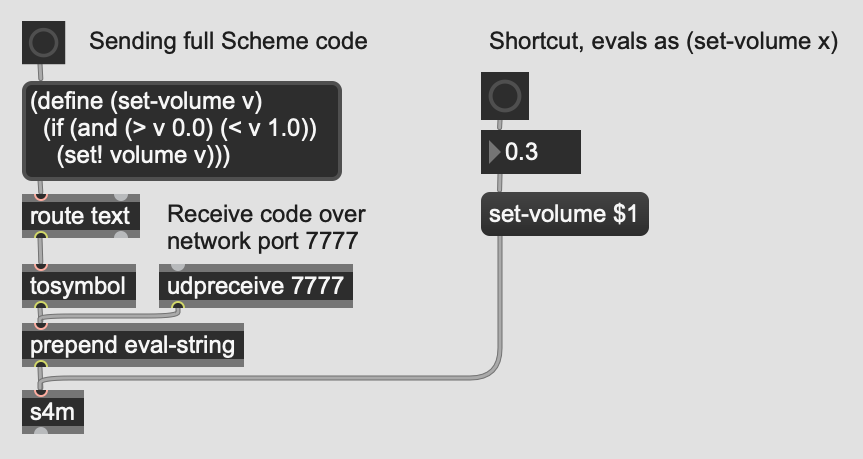
\includegraphics[width=.75\linewidth]{fig-4-code-sends}
  \caption{S4M patch with 3 ways of sending Scheme code to the interpreter}
  \Description{.}
\end{figure}


In addition to both of these, the \textbf{s4m} object implements a \textbf{read} message,
where sending \textbf{read \{filename\} } to the object will result in the full filename
being found on the Max search path and used in a call to the Scheme \textbf{load} function,
without resetting the s7 interpreter.

Taking the above together, we see that users have a wide variety of code input options:
they can change the main file in the \textbf{s4m} box if they want a rebooted interpreter,
they can send \textbf{read} messages if they want to load files without losing 
interpreter state, and they can send code itself either as strings or as Scheme
one-liners implemented as Max messages. The result is that it is straightforward
for users to keep parts of their Scheme program active and running
while working on other parts that are being redefined on the fly (perhaps while music plays!),
a workflow that is very convenient to algorithmic musicians, but impractical with existing
Max options. Of particular note, this enables the user to
conveniently create new functions and schedule them for future evaluation,
as discussed in the next section.


\section{Event scheduling in computer music and Max}

Music is fundamentally a temporal art form --- there may be music with static pitch
or static amplitude, but absent rhythm, there is no music.  
Thus a core problem in computer music programming environments is that of providing a flexible 
means of triggering events in time. Further, in platforms intended to support both
live and algorithmic musical interaction, a viable solution must enable the performer
to interact with scheduled events easily, both programmatically and gesturally. 

One of the major advantages of Max compared to other computer music platforms 
is the ease with which the user can create interactive environments in which the performer's actions 
change musical parameters in complex ways, enabling 
musically rich performances. It is, for example, trivial to add GUI elements to change
musical parameters, and only slightly less trivial to add handlers for MIDI input, 
so that users can connect to their programs physical devices such as
piano-style keyboards, and mixing board knobs, faders, and buttons. 

For performers and composers exploring the intersections of live performance and algorithmic
composition, one is ideally able to use gestural inputs not just to affect
what is happening \textit{now} (as with a traditional musical instrument), but also what will 
happen \textit{in the future}. For example, a performer may have two physical dials,
and may wish to schedule an event in the future that will use parameters derived
from these dials, but may wish one parameter to be used as the dial is now
(at the time of event dispatch) 
and the other to be used as the performer will have the dial at the scheduled time.
Further, the absolute time of the event may not even be known at the time of 
scheduling, as could be the case if the event time was specified in musical terms 
(i.e., on the down-beat of the next 8 bar section) and the tempo might be changed 
prior to the scheduled (musical) time. 

The author proposes that this problem is one not well solved in the Max environment prior 
to Scheme For Max. Max does provide facilities to delay Max messages by some
amount of time. In the context of visual patcher programming, users can schedule 
a Max message (number, symbol, or list of both) for future processing by sending it through a 
\textbf{pipe} object. The amount of time by which it is delayed is specified as an argument to 
the \textbf{pipe} object, and can be expressed in milliseconds or in a tempo 
relative format with the actual time determined by the Max master transport tempo. 
The \textbf{pipe} object’s delay time can also be set dynamically by sending a numerical message
to the right inlet. Any messages sent to the left inlet will be passed out
the outlet(s) after the specified time. 

While moving events into the future with the \textbf{pipe} object is simple to program 
in the patcher and functions adequately, 
it has several limitations. The most immediately noticeable is that it also splits 
list messages into individual elements, sending them out individual outlets. 
If the user wishes to delay a complex event with many parameters, something easily 
expressed in list format, it requires the user to specify how many atoms will 
be in an incoming list message in advance and to reassemble the message manually.
If the length of the list is unknown (i.e., the event uses an arbitrary number
of parameters), the solution is more complex and requires 
an exterior storage mechanism to be used to allow the outgoing 
message to re-fetch the original list from another object after delay. Using
the \textbf{pipe} object for delaying complex events is thus cumbersome. 

A larger problem is that of how to capture gestural values for use in the delayed
events. Max's visual patching language is fundamentally modelled similarly to a modular
synthesizer --- there is one instance in memory of each visual object, and messages can only
pass through them one at a time. Creating visual programs where execution of 
delayed events will trigger cascades of messages through objects that are also 
being used in the interim becomes onerously complex and there exists no straightforward
facility to express \textit{``make a new container for this variable as it is now so that
we can fetch it later"}. A naive solution would be to use a visual patcher object to store 
the variable's state at trigger time for use later, however this only works
if there is only one scheduled event --- adding more scheduled events requires adding
an additional storage objects per concurrently scheduled event, and as each object in the visual patcher
represents an object instantiation rather than a class, this rapidly becomes
baroque. This ``programming-with-instances" paradigm
is very convenient when we want to ensure there is only ever one instance of a given function, such
as in emulation of a hardware synthesizer, where each oscillator represents one ``always-on"
physical device that is playing regardless of whether one can hear it. 
However, it is difficult in a polyphonic time context
such as the creation and eventual playback of some arbitrary number of delayed events.

\begin{figure}[H]
  \centering
  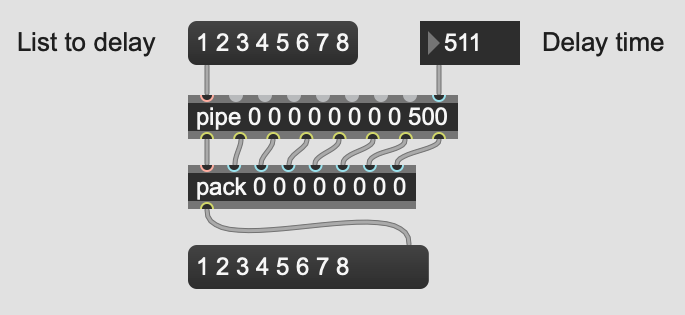
\includegraphics[width=.5\linewidth]{fig-5-pipe}
  \caption{Delaying a list message with the pipe object requires reassembling the list with the pack object}
  \Description{.}
\end{figure}

It should also be mentioned that there exists within Max a facility for creating
new instances of Max sub-patches on demand, designed with the express purpose of
overcoming this barrier. One can use the \textbf{poly} object to create polyphonic
patches. However, this involves complex patching, so we will not examine this further here,
save to comment that this again becomes cumbersome when dealing
with a potentially large and unknown number of events, each with arbitrary numbers
of parameters.

In the C API however, Max does provide a highly accurate facility for delaying
the execution of a C callback function, through the Max \textbf{clock} API. Scheme
for Max builds on this to provide an accurate, flexible, and high-level means 
to schedule future events, without the problems described.

\section{Comparison with the Max JavaScript object}

We can see that the visual patching language of Max is not well suited to implementing
our use case of a performer wanting to schedule large numbers of events with arbitrary numbers of
parameters and gestural inputs meant variously for present and future use. 
However, Max does provide an alternative programming solution through its
\textbf{js} object, which embeds a JavaScript (ECMA5) interpreter in the Max environment.
The user is able to load JavaScript code from a file (provided as an argument to the object),
and this code can interact with the Max environment and with object inlets and outlets,
similar to how one can do so in C code in a Max external.
This does allow one to create functions and variables, and does have a facility
for delayed execution through the JavaScript \textbf{Task} object. 
Thus technically it could be used to solve our use case.
In many respects the \textbf{js} object is functionally similar to the \textbf{s4m} object,
and in fact, the desire to work with Max this way, but without the limitations of the Max
JavaScript implementation, was the reason for the development of S4M.

The \textbf{js} object in Max is not an ideal solution to our problem for several reasons. 
The most serious is that it is limited to running only in the Max low-priority GUI thread \cite{Cycling74}.
As this thread is also used for Max file i/o and graphic redrawing, the result is that latency
is potentially high and indeterminate, meaning musical timing accuracy is unpredictable and often poor.
The human ear is very sensitive to time, with delays of tens of milliseconds being enough to sound like errors in playback
of highly rhythmic music. This means that it takes little other activity in the
GUI thread to delay our scheduled events enough to be audibly incorrect. 
For some purposes, this is acceptable, but for the creation of accurate 
musical sequencers or algorithmic music engines, the \textbf{js} object is unreliable. 

Secondly, the \textbf{js} object provides no convenient facilities for loading new code
during playback such as was previously described for S4M.
The object reads in a single source file at instantiation time.
One could technically add dynamic code evaluation by wrapping
code to be evaluated in strings and passing this message to a JavaScript function
that uses the JavaScript \textbf{eval} function, much as S4M does with the
\textbf{eval-string} message. However, this pattern is not common and well-supported
in the JavaScript milieu the way it is in Lisp languages, as it poses a serious security risk in a 
web development context, which is the use case driving JavaScript linguistic
evolution, literature, and tooling.

Finally, the \textbf{js} object gives us JavaScript's implementation of anonymous functions
and closures, which while usable, are verbose in terms of syntax, and require
diacritical syntax that is not easily used in Max messages. When compared to the syntax
of Scheme, JavaScript is thus impractical for generating code in Max messages.

This is of particular significance to algorithmic performers, 
for example in the live-coding scene, who might
want to not just schedule a pre-written function, but create a new function 
and schedule it while a piece plays.


\section{Scheduling events in Scheme For Max}

Given the above, we can see that the problem of elegantly implementing 
a delayed event system that can differentiate between current and future values
for variables derived from real-time input gestures is well suited to solutions 
using Scheme. Scheme is notable for the conciseness with which one can create an anonymous function
and store a reference to this function (taking along its environment) in some data
store to be retrieved at an arbitrary point in time. Further, it is straightforward
to differentiate in the function between variables that should
be used with their value as they are at function definition time versus
as they are at eventual evaluation time. The underlying host system is required only to 
implement the ability to execute a callback at some time in the future, so long as 
the callback has a means to retrieve some reference to the function stored.
Scheme For Max brings this facility to the Max environment.

\begin{figure}[H]
  \centering
  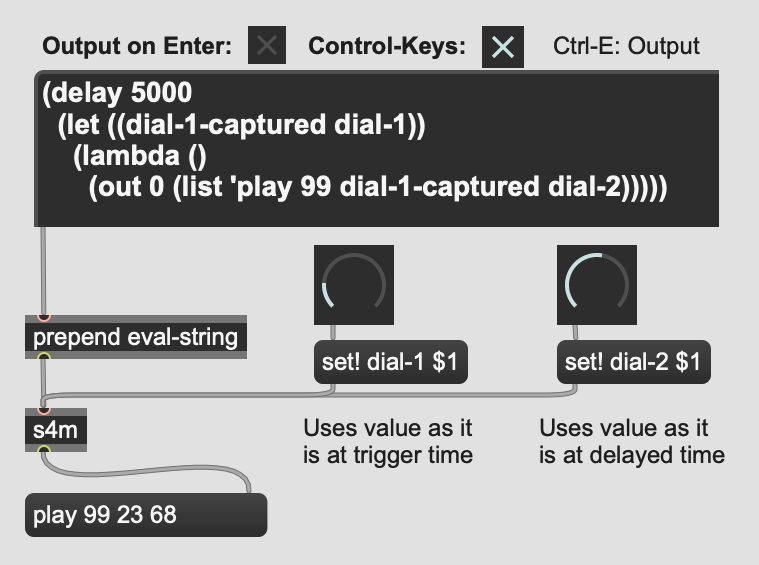
\includegraphics[width=.5\linewidth]{fig-6-s4m-delay}
  \caption{Delaying a mixed list message, with dial values used with present and future values}
  \Description{.}
\end{figure}

\subsection{Clock Implementation in Max}

To discuss the implementation of scheduled functions in S4M, we must first examine
briefly the implementation of Max externals in C and the aforementioned 
facilities for delaying functions.

At a high level, a Max external must implement the following:

\begin{itemize}
\item A data structure to hold state used by the object
\item A class-building function used to create the class in C
\item An instance constructor function called when objects are added to a patch
\item Any methods that will be bound to messages as event handlers
\end{itemize}

A sample of code for a minimal external is shown below,
for an object called \textbf{mynum}. The object holds an integer as state,
updates the integer on receipt of an \textbf{int} 
message, and posts the value to the console on receipt of a \textbf{bang}
message.

\begin{lstlisting}[language=C]

// data structure of instance fields for our class
typedef struct _mynum {
    t_object obj;     // obligatory member for the mynum instance 
    long value;       // state variable for the integer
} t_mynum;

// global pointer to our class definition that is setup in ext_main()
static t_class *mynum_class; 

// ext_main, the obligatory setup function that builds the mynum class
void ext_main(void *r){
    t_class *c;
    c = class_new("mynum", (method)mynum_new, (method)NULL, sizeof(t_mynum), 0L, 0);
    // bind handlers for the messages we want to be able to receive
    class_addmethod(c, (method)mynum_int, "int", A_LONG, 0);
    class_addmethod(c, (method)mynum_bang, "bang", NULL, 0);
    class_register(CLASS_BOX, c);
    mynum_class = c;
}

// constructor for our object
// the value returned by the below gets stored in the obj field of our t_mynum struct
void *mynum_new(){
    // pointers to the object defined are traditionally called "x"
    t_mynum *x = (t_mynum *)object_alloc(mynum_class);
    x->value = 0;
    return x;
}

// a method handler for int messages that updates the internal state
void mynum_int(t_mynum *x, long n){
    x->value = n;
}

// a method handler for bang messages, post the internal int to console
void mynum_bang(t_mynum *x){
    post("value is %ld",x->value);
}

\end{lstlisting}


We can see that the pattern for adding functionality to our class is to
add state variables to the \textbf{t\_mynum} structure, and add methods as
functions expecting a pointer to our object as the first argument,
traditionally named ``x". In the example above, a \textbf{bang} message causes our
object to run, with the side effect of posting the stored value to the console. A more
realistic example would likely output the stored value, but this adds more code
and is not necessary for our demonstration of scheduling.

Let us imagine instead that the \textbf{bang} message should delay the activity
of posting to the console by 1000 ms. We can use the Max \textbf{clock} facility for high-accuracy
delay, as it accepts floats for the ms time value. (Note that the actual delay time
will be offset to the nearest signal vector boundary, determined by the
users ``Signal Vector Size" audio setting, but subsequent clock calls 
adjust for this, maintaining long-term temporal accuracy. If one needs
single-sample accuracy, the solution is to simply set the signal vector to a size of 1.)  

We will create a \textbf{clock} object, which takes as arguments a void pointer and a function
reference, with the void pointer normally used to hold a reference to our instantiated
object (x). The standard method for doing this in Max (taken from the SDK documentation)
is to add a \textbf{clock} object to our class's data structure, and to add the act
of starting the clock to the \textbf{bang} handler.

\begin{lstlisting}[language=C]
// typical Max clock use

typedef struct _myint {
    t_object  obj;          // member for the actual instance 
    long      value;        // state variable for the integer
    void      *clock;       // will hold clock pointer
} t_myint;

// update the constructor to make a clock
void *myint_new(){
    t_myint *x = (t_myint *)object_alloc(myint_class);
    x->value = 0;
    // create a clock bound to the myint_callback method
    x->clock = clock_new(x, (method)myint_callback); 
    return x;
}

// update the bang handler to start the clock
void myint_bang(t_myint *x){
  clock_fdelay(x->clock, 1000);
}

// the callback that will be triggered by the clock
void myint_callback(t_myint x){
    post("in the future, the value is %ld",x->value);
}
\end{lstlisting}


From the above we can see that, while accurate, the clock functionality is limited ---
the callback must be a single-arity function expecting a pointer, and this
is normally a pointer to the object.


\subsection{Implementation in Scheme For Max}

Scheme For Max builds on the clock facility provided by the Max API to allow scheduling
Scheme functions. The delayed functions are limited to zero-arity signatures, but as
creation of lambda functions in Scheme is trivial, this is of little practical significance to 
user. To the user of S4M, scheduling the execution of a function is simple:

\begin{lstlisting}[language=lisp]
; schedule a function for 1000 ms in the future
; it will send the int 99 out outlet 0 of the s4m object
(delay 1000 (lambda()(out 0 99)))
\end{lstlisting}

In addition to scheduling the function, \textbf{delay} also returns a unique
symbolic handle representing the scheduled instance, and this can be used to 
cancel the execution of the scheduled function.

\begin{lstlisting}[language=lisp]
; delay and store the handle
(define handle 
  (delay 1000 (lambda()(out 0 99))))

; cancel it
(cancel-delay handle)
\end{lstlisting}

The Scheme implementation of this is straightforward:

\begin{itemize}
\item The \textbf{delay} function (in Scheme) creates a unique symbolic handle, and stores the 
  function passed to it in a hash-table, keyed by this handle.
\item It then calls \textbf{s4m-schedule-delay}, which is implemented
  in C and takes as arguments the delay time and the symbolic handle. It will handle 
  clock creation.
\item When the clock callback runs after the time has elapsed, it calls (from C) the Scheme function 
  \textbf{s4m-execute-callback}, which uses the handle received as an argument 
  to retrieve the delayed function from the Scheme hash-table and call it.
\end{itemize}

Cancelling a delay function consists of merely replacing the callback registered
in the hash-table with the value \textbf{\#false}, letting the clock fire harmlessly.
The s7 Scheme code for this is shown below. It uses an s7's \textbf{gensym} function to create a
symbolic handle that is guaranteed to be unique to this instance of the interpreter.

\begin{lstlisting}[language=lisp]

; registry of delayed functions, by handle 
(define s4m-callback-registry (hash-table))

; function to register a callback by a handle and return handle
(define (s4m-register-callback cb-function)
  (let ((key (gensym)))
    (set! (s4m-callback-registry key) cb-function)
    key))

; fetch a callback from the registry 
(define (s4m-get-callback key)
  (let ((cb-function (s4m-callback-registry key)))
    cb-function))

; internal function to get a callback from the registry and run it
; this gets called from C code when the Max clock fires
(define (s4m-execute-callback key)
  ; get the func, note that this might return false if was cancelled
  (let ((cb-fun (s4m-get-callback key)))
    ; de-register the handle
    (set! (s4m-callback-registry key) #f)
    ; if callback retrieval got false, return null, else execute 
    (if (eq? #f cb-fun) 
      '()
      ; call our cb function, catching any errors here and posting
      (catch #t 
        (lambda () (cb-fun)) (lambda err-args (post "ERROR:" err-args))))))

; public function to delay a function by time in ms (int or float)
; returns the gensym callback key, which can be used to cancel it
(define (delay delay-time fun)
  ; register the callback and return the handle
  (let ((cb-handle (s4m-register-callback fun)))
    ; call the C FFI and return the handle
    (s4m-schedule-delay delay-time cb-handle)
    cb-handle))

\end{lstlisting}

The functions prefixed with \textbf{s4m-} are internal; the S4M user 
need only understand how to call the \textbf{delay} function.

The implementation in C is more involved to work around the signature 
limitations of the clock facilities in Max.
When the \textbf{s4m-schedule-delay} function is run, receiving the symbolic handle
and delay time as arguments, the following occurs:

\begin{itemize}
\item A \textbf{t\_s4m\_clock\_callback} data structure is dynamically allocated and used to store a
  reference to the \textbf{s4m} object and to the symbolic handle passed from Scheme.
\item A Max \textbf{clock} is created, passing in a void pointer to a clock callback structure
  and binding the clock to a generic clock callback function in C. The clock's timer is started.
\item The clock callback struct is also stored in a C hash-table (using Max's \textbf{hashtab} implementation),
  keyed by the handle, so that cancellation or object deletion can use this to find all clocks.
\item When the generic clock callback function runs (time has elapsed), it uses the pointer argument to get 
  the delay handle and the instantiated \textbf{s4m} object, through which it 
  can also get the s7 interpreter pointer.
\item The s7 interpreter and handle are then used to call the Scheme function
  \textbf{s4m-execute-callback,} which will run our delayed Scheme function as previously explained.
\item The generic C callback then removes the clock reference from the C hash-table,
  deletes the clock, and frees the memory allocated for the callback struct.
\end{itemize}

Additionally, there exists clean up functionality triggered on a \textbf{reset} message or 
\textbf{s4m} object destruction which fetches from the hash-table all outstanding clocks, 
cancels them, and frees the memory allocated.
This is not shown as it does not materially change the process used.

\begin{lstlisting}[language=C]

// the struct for the s4m object, with most elements removed
typedef struct _s4m {
    t_object obj;
    // pointer to the s7 interpreter (initialization of which is not shown)
    s7_scheme *s7;
    // a Max hash table for storing clocks (for reset clean-up)
    t_hashtab *clocks;     
} t_s4m;

// the clock callback struct
typedef struct _s4m_clock_callback {
   t_s4m obj;
   t_symbol *handle; 
} t_s4m_clock_callback;

// schedule delay FFI definition, called from Scheme as s4m-schedule-delay
static s7_pointer s7_schedule_delay(s7_scheme *s7, s7_pointer args){
    // as this is called from Scheme, we must find x by fetching it
    // from the Scheme variable set in initialization
    t_s4m *x = get_max_obj(s7);

    // get the arguments we need (time and handle) from the s7 args list
    // that represents the arguments passed to s4m-schedule-delay in Scheme
    // first arg is float of time in ms 
    double delay_time = s7_real( s7_car(args) );

    // second arg is the symbolic handle
    char *cb_handle_str;
    s7_pointer *s7_cb_handle = s7_cadr(args);
    cb_handle_str = s7_symbol_name(s7_cb_handle);

    // allocate memory for our clock_callback struct and populate
    // NB: this gets cleaned up by the receiver in the clock callback above
    t_s4m_clock_callback *clock_cb_info = 
        (t_s4m_clock_callback *)sysmem_newptr(sizeof(t_s4m_clock_callback));
    clock_cb_info->obj = *x;
    clock_cb_info->handle = gensym(cb_handle_str);

    // make a clock, setting our callback info struct as the owner, as a void pointer
    // when the callback method fires, it will retrieve this pointer as an arg 
    // and use it to get the handle for calling into scheme  
    void *clock = clock_new( (void *)clock_cb_info, (method)s4m_clock_callback);

    // store the clock ref in the s4m clocks hashtab (used to get at them for reset cancelling) 
    hashtab_store(x->clocks, gensym(cb_handle_str), clock); 

    // schedule it, this is what actually kicks off the timer
    clock_fdelay(clock, delay_time);

    // return the handle to the Scheme caller
    return s7_make_symbol(s7, cb_handle_str);
}

// the generic clock callback, this fires after being scheduled with clock_fdelay 
// it gets access to the handle and s4m obj through the clock_callback struct
// this is the C callback that runs for every delayed Scheme function 
void s4m_clock_callback(void *arg){
    t_s4m_clock_callback *ccb = (t_s4m_clock_callback *) arg;
    t_s4m *x = &(ccb->obj);
    t_symbol handle = *ccb->handle; 
  
    // call into Scheme with the handle, where Scheme will call the registered delayed function
    // we must build a Scheme list through the FFI to use as the arguments
    s7_pointer *s7_args = s7_nil(x->s7);
    s7_args = s7_cons(x->s7, s7_make_symbol(x->s7, handle.s_name), s7_args); 

    // call the Scheme s4m-execute-callback function
    // s4m_s7_call is a simple wrapper around s7's s7_call with error handling and logging 
    s4m_s7_call(x, s7_name_to_value(x->s7, "s4m-execute-callback"), s7_args);   

    // remove the clock(s) from the clock registry and free the cb struct
    hashtab_delete(x->clocks, &handle);
    // free the memory for the clock callback struct 
    sysmem_freeptr(arg);
}

// clean up methods for s4m reset and delete not shown

\end{lstlisting}

\section{Limitations and Future Improvements}

The scheduling system describe does have several limitations worth noting.
The s7 Scheme implementation includes a tracing garbage collector 
that must run occasionally, pausing other processing \cite{Matheussen2020}.
The garbage collector can, however, be paused and run on demand. Tests on the author's
system, with the garbage collector forced to run every 100 ms to prevent
significant build up, showed the garbage collection taking an average of 1 to 2 ms per pass
when run in a substantial application (a 16 track sequencer written entirely in S4M
with the computer also generating audio for the tracks with commercial
software synthesizers).  
The audio rendered was recorded and examined
in a digital audio workstation to check for timing discrepancies. The
results of these preliminary tests were that timing was unaffected by the 
garbage collector so long as Max was configured with 
a large enough output buffer to allow the collector to run within the 
latency period of this buffer.
Using Max with an output buffer of 256 samples produces an output latency
of approximately 6-8 ms (depending on the Max signal vector as well), which
was large enough for the collector to run without issue, but is 
low enough to be acceptable for real-time performance. With software synthesis
loads at closer to the maximum possible on the author's computer,
an output buffer of 512 samples (approx. 11 ms output latency) was necessary to prevent
any timing errors. This is encouraging as these buffer sizes are not atypical
for commercial music production on digital audio workstations and are widely
considered as being in acceptable ranges for real-time music systems \cite{Brandt1998}.

In addition to output latency, there is the factor of internal latency.
Max, like many computer music programming environments, generates audio 
in vectors of samples, with
each vector generated from one processing pass, and (normally) control
rate passes conducted also a maximum of once per audio vector pass \cite{Puckette2002}.
The size of this signal vector thus has a large effect on performance, with larger
vectors requiring significantly less CPU use. As audio rendering of note onsets originating
from control messages (the normal scenario) must thus be aligned with 
signal vector boundaries, this produces delays of note onsets by up to
the time period of one vector, a phenomenon known as ``timing jitter" in the nomenclature.
However, the more recent scheduling facilities in Max, including the 
clock facilities used by S4M, are implemented to compensate for this jitter,
maintaining long-term temporal accuracy despite note onset delays. The mechanism
by which this is done is unfortunately not publicly documented or available
in open-source code, but one can assume that it is some variant of the common pattern 
whereby scheduled events are aware of when they are supposed to be running
(``logical-time"), and if they in turn schedule subsequent events, the time for these subsequent
events will be shifted to compensate for the jitter, based 
on the logical time of the scheduling event, rather than its
actual (post-jitter) actual clock time \cite{Anderson1986}.
The author also conducted personal tests of 
this compensation, comparing both high and low signal vector sizes to produce
variable delays in note onsets, and it was determined
that so long as the overall output latency is again large enough to allow
the GC to run in time, self-scheduling events in a long piece do stay
accurate in that jitter does not accumulate over the piece (note onsets 
stay accurate to within the delay of one signal vector of samples,
regardless of the length of the piece of music).

These tests demonstrated that Scheme For Max is usable as a highly accurate
timing source for processing-intensive music production so long as some
reasonable latency is used, but that at low latencies the garbage
collector will interfere with timing by generating audio under-runs.
Improving or replacing the s7 garbage collection implementation for 
lower latency use is a potential area for future work. 

A second limitation is that S4M does not implement DSP calculations at this
time, running only in the Max event/message thread. 
Max does have an audio configuration option
whereby the event thread and DSP thread are shared in a round-robin
execution pattern. It is worth exploring whether the Scheme interpreter
could be run productively in the DSP loop in this configuration. While it is
unlikely that S4M will be suitable for processing-intensive audio synthesis
(requiring filling the whole vector per pass), it is possible that
other productive work could be done once per DSP pass.
This could be used to create the equivalent in Max of the ``control-rate"
as it is implemented in Csound, where rather than control rate calculations being triggered
solely by events, there is also the facility to create lower resolution
continuous signals that can be used to modulate audio signals. 
This can be useful for automating parameters that 
sound acceptable at lower sample rates, such as pitch curves, and is
an area that will be explored in subsequent work on S4M.


\section{Conclusion}
The Scheme For Max project brings a new way of working 
to the Max platform, especially with regard to flexible and accurate 
scheduling of future events.  The author believes this will be
of significant benefit to those working in the fields of algorithmic
music and live coding, and will also be useful to the more general Max 
user base as a way to script Max in a high-level language that runs in
the high-priority thread. In the author's experience, 
working in Scheme within Max has been highly productive, with the
language well suited both to expressing musical concepts and to working
with the Max platform. The ability to update code during play-back
has been an especially productive workflow for building complex 
sequencing and algorithmic composition tools.

Future plans for the project include a version for the open-source
Pure Data platform, similar to Max in many ways and created also by Miller Puckette,
the original author of Max. \textbf{Scheme For Pure Data} is now in beta release, available
as source code, with binary releases planned for August 2021. In addition
to this, experimental work on running Scheme for control-rate DSP is planned.
This would entail Scheme executing in the timed audio rendering thread, but
at a subdivision of the audio sample rate such as every 32 or 64 samples, 
thus generating streams similar to the way digital audio is rendered, but
at a lower resolution suitable for use as signal modulators. 

The author also plans to create portability layers in Scheme to allow one to run 
the same Scheme code on S4M, S4Pd, or Common Music (which also uses s7),
and potentially in C++ projects through the JUCE audio development framework.
There have also been successful ports of s7, Pure Data, and Csound to Web Assembly, 
thus it seems likely that work from the project will be useable for web audio as well.
It is hoped that through these additional run-times the project can become 
a valuable addition to the larger computer music community, enabling
use in contexts where the commercial Max platform is not practical
or financially accessible.

As s7 Scheme is open-source itself, another potential area of work
is improving s7's suitability for real-time use. This could include
implementation of an incremental garbage collector, for example.

Scheme For Max can be obtained on GitHub, with links to documentation,
demonstration videos, and various tutorials linked from the main page.

https://github.com/iainctduncan/scheme-for-max
%%
%% The acknowledgments section is defined using the "acks" environment
%% (and NOT an unnumbered section). This ensures the proper
%% identification of the section in the article metadata, and the
%% consistent spelling of the heading.
\begin{acks}
Scheme For Max would not exist without the work of many people. 
Bill Schottstaedt created Common Lisp Music and the s7 Scheme implementation,
and has been invaluable as a source of advice and technical assistance. Heinrich Taube
created Common Music and has been an inspiration through his seminal book
on algorithmic composition with Lisp, ``Notes from the Metalevel".
Luigi Castelli and Alex Harker helped with Max external programming questions
and build assistance. 
S4M of course depends on Max and thus owes a huge debt to 
Miller Puckette and David Zicarelli.
George Tzanetakis, my supervisor, assisted with this paper.
And finally, Andrew Schloss, my other supervior, has
been a source of encouragement and support through the years of 
exploration that led to the Scheme For Max project.

\end{acks}


%%
%% If your work has an appendix, this is the place to put it.
%%
%% The next two lines define the bibliography style to be used, and
%% the bibliography file.
\bibliographystyle{ACM-Reference-Format}
\bibliography{iduncan-icfp21}

\end{document}
\endinput
%%
%% End of file `sample-acmsmall.tex'.




